\documentclass[conference]{IEEEtran}
\IEEEoverridecommandlockouts

\usepackage{cite}
\usepackage{amsmath,amssymb,amsfonts}
\usepackage{algorithmic}
\usepackage{graphicx}
\usepackage{textcomp}
\usepackage{xcolor}
\usepackage{booktabs}
\usepackage{url}
\usepackage{tikz}
\usetikzlibrary{shapes,arrows.meta,positioning,calc}

\def\BibTeX{{\rm B\kern-.05em{\sc i\kern-.025em b}\kern-.08em
    T\kern-.1667em\lower.7ex\hbox{E}\kern-.125emX}}

\begin{document}

\title{Adaptive Behavioral Deception-Resistant Insider\\
Threat Detection Using Counterfactual Digital\\
Twins\\
{\footnotesize \textsuperscript{*}Department of Computer Science and Engineering, Final Year Major Project}
}

\author{\IEEEauthorblockN{Dr. RAJENDRAN T}
\IEEEauthorblockA{\textit{Department of CSE(S)} \\
\textit{Vel Tech Rangarajan} \\
\textit{Dr. Sagunthala R\&D Institute} \\
\textit{of Science and Technology} \\
Chennai, India \\
email@veltech.edu.in}
\and
\IEEEauthorblockN{HARITHA D (VTU24553)}
\IEEEauthorblockA{\textit{Department of CSE(CS)} \\
\textit{Vel Tech Rangarajan} \\
\textit{Dr. Sagunthala R\&D Institute} \\
\textit{of Science and Technology} \\
Chennai, India \\
vtu24553@veltech.edu.in}
\and
\IEEEauthorblockN{MAHISHA V (VTU25143)}
\IEEEauthorblockA{\textit{Department of CSE(CS)} \\
\textit{Vel Tech Rangarajan} \\
\textit{Dr. Sagunthala R\&D Institute} \\
\textit{of Science and Technology} \\
Chennai, India \\
vtu25143@veltech.edu.in}
}

\maketitle

\begin{abstract}
Insider threats represent one of the most critical vulnerabilities in modern enterprise cybersecurity because malicious operators already possess authorized credentials and routine access privileges. While User and Entity Behavior Analytics (UEBA) systems leverage unsupervised anomaly detectors, such as Isolation Forests, they confront a fundamental operational dilemma in dynamic environments. Static detection models fail to accommodate benign operational evolution, causing excessive false positive rates. Conversely, naive adaptive models employing exponential moving average (EMA) updates are vulnerable to adversarial concept drift---a gradual deception and baseline poisoning strategy where adversaries incrementally escalate anomalous activities to blend into the shifting baseline. In this paper, we propose an Adaptive Behavioral Deception-Resistant Insider Threat Detection framework powered by Counterfactual Digital Twins (CDT). Our architecture establishes a privacy-preserving behavioral digital twin for each authorized entity, capturing 6-dimensional orthogonal endpoint telemetry verified at the operating system kernel level (via Win32 \texttt{GetDriveTypeW}). The digital twin models expected normative behavior against an unsupervised Isolation Forest ($T = 100$) and tracks multi-vector divergence. When cumulative feature deviation crosses an empirical statistical threshold ($\sum_{j=1}^6 |Z_j| \ge 4.5$), an automated persistence lock freezes the counterfactual baseline, permanently preventing adversary-induced model poisoning while preserving legitimate drift adaptation and enabling counterfactual ``What-If'' scenario evaluations. Rigorous empirical validation over 30 independent trials across four drift stress levels confirms that under severe adversarial drift ($\Delta_{VH}$), the proposed counterfactual framework sustains an F1-score of $0.968 \pm 0.023$ and a detection rate of $96.1\%$, compared to $0.503$ achieved by the naive adaptive baseline ($p = 0.0001$, paired $t$-test). Furthermore, the architecture complies strictly with GDPR Article 5 by inspecting only non-invasive endpoint operational metadata.
\end{abstract}

\begin{IEEEkeywords}
Insider Threat Detection, Counterfactual Digital Twins, User and Entity Behavior Analytics (UEBA), Concept Drift, Isolation Forest, Adversarial Poisoning, Endpoint Telemetry.
\end{IEEEkeywords}

\section{Introduction}
Modern enterprise cybersecurity perimeters face unprecedented risks from insider threat vectors. Recent cybersecurity industry surveys indicate that insider incidents have risen by more than 44\% across global sectors, with annual containment and incident recovery expenditures exceeding \$15 million per organization \cite{b1}. Unlike external adversaries who must identify and breach perimeter defenses, malicious insiders---encompassing disgruntled employees, compromised service identities, and internal data brokers---operate from within the trust boundary. They possess legitimate cryptographic credentials, authorized system accounts, and routine access to proprietary databases and file repositories \cite{b2}.

Because an insider's malicious operations closely mimic legitimate administrative or business workflows, legacy perimeter defenses---including next-generation firewalls, signature-driven endpoint protection platforms, and rigid threshold alerts---fail to detect sophisticated internal attacks \cite{b2}. To bridge this defense gap, enterprise security operations have increasingly adopted User and Entity Behavior Analytics (UEBA) frameworks. UEBA systems model historical employee activity using unsupervised machine learning algorithms, notably Isolation Forests \cite{b4}, which isolate anomalies efficiently without requiring pre-labeled attack corpora.

Nevertheless, operational deployments of UEBA encounter a severe structural conflict termed the \textit{adaptation-poisoning dilemma} \cite{b5}. In genuine enterprise environments, employee working patterns fluctuate continuously as project assignments shift, organizational restructuring occurs, and seasonal workloads intensify. A strictly \textit{static} anomaly detection engine that locks baseline parameters at deployment cannot accommodate benign operational evolution, resulting in an unsustainable volume of false positive alarms that overwhelms Tier-1 Security Operations Center (SOC) analysts.

Conversely, if the analytics engine deploys a \textit{naive adaptive} update rule---such as incrementally recalculating feature means through an Exponential Moving Average (EMA) or sliding observation window---it introduces an insidious vulnerability known as \textit{adversarial concept drift} or a ``boiling-frog'' poisoning attack \cite{b6}. A patient insider can deliberately pace their illicit actions, exfiltrating small increments of sensitive files and network payloads over weeks or months. Under naive adaptation, each subtle increment shifts the detector's normative mean vector upward, steadily training the model to accept high-volume exfiltration as normal background behavior. When the critical mass of data is finally transferred, the poisoned model treats the event as benign, causing catastrophic detection failure \cite{b8}.

To resolve this challenge, this paper introduces an end-to-end \textbf{Adaptive Behavioral Deception-Resistant Insider Threat Detection Framework Powered by Counterfactual Digital Twins (CDT)}. The primary contributions of this work are summarized as follows:
\begin{enumerate}
    \item \textbf{Kernel-Verified Endpoint Telemetry Sensor:} We implement a low-overhead host telemetry agent that captures authentic process life cycles, delta egress bytes, and physical removable storage attachments verified directly through operating system kernel calls (\texttt{GetDriveTypeW}), eliminating synthetic noise from mapped network drives.
    \item \textbf{Counterfactual Digital Twin Behavioral Modeling:} We formulate a digital twin architecture that synthesizes normative behavior and tracks standardized multi-attribute divergence ($D_t$) over an orthogonal 6-dimensional representation. When composite drift crosses an empirical statistical threshold ($D_t \ge 4.5$), the twin's persistence lock halts adversarial baseline poisoning while preserving legitimate drift adaptation and enabling counterfactual ``What-If'' evaluations.
    \item \textbf{Comprehensive 30-Trial Empirical Validation:} We perform extensive statistical evaluation over 30 independent multi-day simulation trials across four drift stress levels ($\Delta_L, \Delta_M, \Delta_H, \Delta_{VH}$). Paired two-tailed $t$-tests ($p < 0.001$) confirm that the proposed counterfactual framework delivers statistically significant resilience against poisoning compared to naive adaptive architectures.
    \item \textbf{Privacy-Preserving and Explainable Architecture:} In strict accordance with GDPR Article 5 and CCPA standards, our methodology collects zero document body contents, keystroke logs, or desktop captures, while providing transparent feature attribution narratives for SOC analysts.
\end{enumerate}

\section{Related Work}

\subsection{Insider Threat Detection and UEBA Architectures}
Traditional insider threat detection relied on signature-based Intrusion Detection Systems (IDS) and deterministic Security Information and Event Management (SIEM) correlation rules \cite{b2}. While effective against known syntax patterns, rule-based systems are brittle against novel or subtle insider evasion tactics. Modern security paradigms have therefore shifted toward data-driven UEBA architectures leveraging machine learning \cite{b3}. 

Supervised classifiers often struggle in operational settings due to extreme class imbalance and the lack of labeled ground-truth insider attack records. Consequently, unsupervised techniques---including autoencoders, One-Class Support Vector Machines (OC-SVM), and tree ensembles---have become standard \cite{b7}. Liu et al. introduced the Isolation Forest algorithm \cite{b4}, demonstrating that anomalies are structurally susceptible to isolation via random recursive hyper-plane partitioning. Isolation Forests achieve linear computational complexity $O(n \log n)$ and minimal memory footprint, making them uniquely suited for high-throughput host telemetry processing. Recent extensions incorporate deep representations \cite{b9}; however, these approaches typically assume static feature distributions and remain vulnerable to gradual baseline shifts.

\subsection{Concept Drift and Adversarial Baseline Poisoning}
Concept drift denotes unpredictable variations in statistical data properties over time ($P_t(\mathbf{X}, y) \neq P_{t+1}(\mathbf{X}, y)$) \cite{b5}. In cybersecurity telemetry, drift manifests across two distinct categories: \textit{benign operational drift} (e.g., changes in team deliverables or working hours) and \textit{adversarial concept drift} (deliberate evasion tactics where adversaries pollute learning parameters) \cite{b6}. 

Kloft and Laskov provided foundational theoretical analyses of online learning vulnerabilities under poisoning attacks, proving that unconstrained parameter updates inevitably guarantee bounded evasion for persistent adversaries \cite{b8}. Existing mitigation strategies have explored dual-memory ensembles, decaying sliding windows, and statistical drift detectors such as DDM and EDDM \cite{b5}. Nevertheless, conventional drift detectors are primarily tuned to detect sudden distribution shifts, often failing to differentiate multi-vector coordinated exfiltration from benign single-feature drift. Our work addresses this gap by introducing an explicit composite $Z$-score persistence lock coupled directly with an unsupervised isolation ensemble.

\section{System Architecture and Threat Model}

\subsection{Threat Model and Operational Assumptions}
We consider a realistic enterprise operational scenario involving a semi-honest or rogue insider operating an authorized workstation. The insider possesses valid directory credentials, administrative execution privileges on their local machine, and routine read access to proprietary project repositories. The adversary possesses basic knowledge of enterprise security auditing and purposefully seeks to exfiltrate confidential intellectual property without triggering static volumetric threshold alarms. 

The attacker adopts a ``low-and-slow'' exfiltration pacing strategy: transferring files in modest batches during off-hours, staging compressed archives in user-level directories, and connecting physical USB mass storage devices. Under conventional adaptive UEBA, such gradual activity aims to gradually shift normative behavioral baselines over several weeks.

\subsection{Distributed System Architecture}
As illustrated in Fig.~\ref{fig:arch}, our system employs a modular, decoupled four-tier microservices architecture designed for resilience, horizontal scalability, and low endpoint overhead:

\begin{figure}[htbp]
\centering
\resizebox{\columnwidth}{!}{%
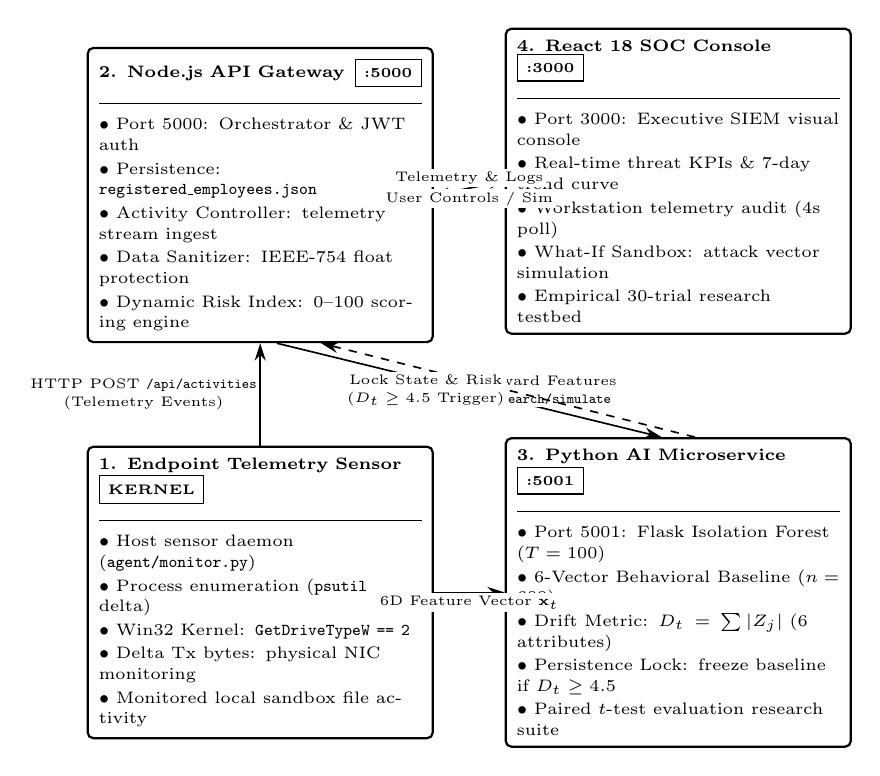
\begin{tikzpicture}[
    node distance=1.3cm and 0.8cm,
    tierbox/.style={
        draw=black,
        line width=0.8pt,
        rounded corners=2pt,
        fill=white,
        text width=4.1cm,
        inner sep=4pt,
        font=\fontsize{6.5pt}{7.5pt}\selectfont,
        align=left
    },
    arrowlabel/.style={
        font=\fontsize{5.5pt}{6.5pt}\selectfont,
        align=center,
        fill=white,
        inner sep=1pt
    },
    conn/.style={
        -{Stealth[length=2.2mm,width=1.4mm]},
        line width=0.6pt,
        draw=black
    },
    biconn/.style={
        {Stealth[length=2mm,width=1.2mm]}-{Stealth[length=2mm,width=1.2mm]},
        line width=0.6pt,
        draw=black
    }
]

% Node 1: Sensor (Bottom Left)
\node[tierbox] (sensor) {
    \textbf{1. Endpoint Telemetry Sensor} \hfill \fbox{\tiny\textbf{KERNEL}}\\[2pt]
    \rule{\linewidth}{0.3pt}\\[2pt]
    $\bullet$ Host sensor daemon (\texttt{agent/monitor.py})\\[1pt]
    $\bullet$ Process enumeration (\texttt{psutil} delta)\\[1pt]
    $\bullet$ Win32 Kernel: \texttt{GetDriveTypeW == 2}\\[1pt]
    $\bullet$ Delta Tx bytes: physical NIC monitoring\\[1pt]
    $\bullet$ Monitored local sandbox file activity
};

% Node 2: Gateway (Top Left)
\node[tierbox, above=1.3cm of sensor] (gateway) {
    \textbf{2. Node.js API Gateway} \hfill \fbox{\tiny\textbf{:5000}}\\[2pt]
    \rule{\linewidth}{0.3pt}\\[2pt]
    $\bullet$ Port 5000: Orchestrator \& JWT auth\\[1pt]
    $\bullet$ Persistence: \texttt{registered\_employees.json}\\[1pt]
    $\bullet$ Activity Controller: telemetry stream ingest\\[1pt]
    $\bullet$ Data Sanitizer: IEEE-754 float protection\\[1pt]
    $\bullet$ Dynamic Risk Index: 0--100 scoring engine
};

% Node 3: AI Service (Bottom Right)
\node[tierbox, right=0.9cm of sensor] (ai) {
    \textbf{3. Python AI Microservice} \hfill \fbox{\tiny\textbf{:5001}}\\[2pt]
    \rule{\linewidth}{0.3pt}\\[2pt]
    $\bullet$ Port 5001: Flask Isolation Forest ($T=100$)\\[1pt]
    $\bullet$ 6-Vector Behavioral Baseline ($n=600$)\\[1pt]
    $\bullet$ Drift Metric: $D_t = \sum |Z_j|$ (6 attributes)\\[1pt]
    $\bullet$ Persistence Lock: freeze baseline if $D_t \ge 4.5$\\[1pt]
    $\bullet$ Paired $t$-test evaluation research suite
};

% Node 4: Console (Top Right)
\node[tierbox, above=1.3cm of ai] (console) {
    \textbf{4. React 18 SOC Console} \hfill \fbox{\tiny\textbf{:3000}}\\[2pt]
    \rule{\linewidth}{0.3pt}\\[2pt]
    $\bullet$ Port 3000: Executive SIEM visual console\\[1pt]
    $\bullet$ Real-time threat KPIs \& 7-day trend curve\\[1pt]
    $\bullet$ Workstation telemetry audit (4s poll)\\[1pt]
    $\bullet$ What-If Sandbox: attack vector simulation\\[1pt]
    $\bullet$ Empirical 30-trial research testbed
};

% Connections
% 1 -> 2
\draw[conn] (sensor.north) -- (gateway.south) 
    node[midway, left, arrowlabel] {HTTP POST \texttt{/api/activities}\\(Telemetry Events)};

% 1 -> 3
\draw[conn] (sensor.east) -- (ai.west) 
    node[midway, below, arrowlabel] {6D Feature Vector $\mathbf{x}_t$};

% 2 <-> 4
\draw[biconn] (gateway.east) -- (console.west) 
    node[midway, above, arrowlabel] {Telemetry \& Logs}
    node[midway, below, arrowlabel] {User Controls / Sim};

% 2 -> 3
\draw[conn] ([xshift=6pt]gateway.south) -- ([xshift=-6pt]ai.north) 
    node[midway, right, arrowlabel] {Forward Features\\\texttt{/research/simulate}};

% 3 -> 2
\draw[conn, dashed] ([xshift=6pt]ai.north) -- ([xshift=22pt]gateway.south) 
    node[midway, left, arrowlabel] {Lock State \& Risk\\($D_t \ge 4.5$ Trigger)};

\end{tikzpicture}%
}
\caption{End-to-End System Architecture: Endpoint Hardware Telemetry Sensor, Enterprise API Gateway, Python Isolation Forest Engine, and Research SOC Console (Rendered in Monochrome/Grayscale).}
\label{fig:arch}
\end{figure}

\begin{enumerate}
    \item \textbf{Kernel-Verified Endpoint Telemetry Sensor (Tier 1):} Implemented as an autonomous background daemon on the monitored host, the sensor collects behavioral telemetry at 3-second sampling intervals. To ensure data authenticity, the sensor interfaces directly with the host operating system kernel:
    \begin{itemize}
        \item \textit{Physical Removable Storage Verification:} Rather than relying on easily spoofed drive letter heuristics, the sensor queries the Win32 API function \texttt{GetDriveTypeW}. Only storage volumes returning return code \texttt{DRIVE\_REMOVABLE} ($= 2$) are tagged as removable physical media, strictly distinguishing flash drives from network mounts (\texttt{DRIVE\_REMOTE} $= 4$) and fixed storage (\texttt{DRIVE\_FIXED} $= 3$).
        \item \textit{Network Egress Monitoring:} Real-time physical network interface queries calculate delta transmission bytes ($\Delta \text{Tx}$) between successive sampling intervals, tracking outbound payload bursts.
        \item \textit{Process Execution Taxonomy:} Active processes are mapped against an enterprise risk categorization hierarchy: benign office productivity (Level 1), development compilers (Level 2), administrative scripting shells such as PowerShell (Level 3), and anonymizing tunneling tools such as Tor or proxy tunnels (Level 4).
    \end{itemize}
    \item \textbf{Enterprise API Gateway (Tier 2):} Built with Node.js and Express.js (Port 5000), this gateway coordinates telemetry ingestion, applies data sanitization to prevent IEEE-754 floating-point exceptions (\texttt{NaN} / \texttt{Infinity}), manages analyst JWT sessions, and maintains an in-memory database fallback to guarantee uninterrupted ingestion during network partition events.
    \item \textbf{Python AI Microservice (Tier 3):} Deployed as a dedicated Flask/Scikit-learn service (Port 5001), this engine houses the Isolation Forest and drift-locking algorithms, exposing REST endpoints for real-time inference (\texttt{/analyze}), health monitoring (\texttt{/health}), and baseline retraining (\texttt{/train-baseline}).
    \item \textbf{Interactive SOC Console (Tier 4):} A modern React 18 dashboard (Port 3000) delivering real-time threat KPIs, 7-day risk trajectories, an employee risk matrix, chronological activity timelines, and an interactive ``What-If'' simulation sandbox for security analysts.
\end{enumerate}

\section{Mathematical Formulation and Methodology}

\subsection{Standardized Behavioral Feature Vector}
At each discrete operational day $t$, the aggregated telemetry for an observed entity is projected into a normalized 6-dimensional feature vector $\mathbf{x}_t \in \mathbb{R}^6$:
\begin{equation}
\mathbf{x}_t = \big[ f_{\text{hour}}, f_{\text{dur}}, f_{\text{app}}, f_{\text{file}}, f_{\text{usb}}, f_{\text{net}} \big]^T
\label{eq:feature_vec}
\end{equation}
where:
\begin{itemize}
    \item $f_{\text{hour}} \in [0.0, 23.9]$ is the initial session login timestamp in decimal hours,
    \item $f_{\text{dur}} \in [0, \infty)$ denotes total active host session duration in minutes,
    \item $f_{\text{app}} \in \{1, 2, 3, 4\}$ indicates the highest process execution risk tier observed,
    \item $f_{\text{file}} \in \mathbb{N}_0$ counts total modified or accessed filesystem objects,
    \item $f_{\text{usb}} \in \{0, 1, 2\}$ reflects physical USB attachment status ($0 = \text{none}$, $1 = \text{authorized peripheral}$, $2 = \text{removable mass storage}$),
    \item $f_{\text{net}} \in [0, \infty)$ measures cumulative outbound network egress in megabytes (MB).
\end{itemize}

\subsection{Unsupervised Isolation Forest Anomaly Scoring}
The reference anomaly detector is trained on an initial historical calibration set of $n = 600$ normal operational vectors. An ensemble of $T = 100$ isolation trees ($\mathcal{T} = \{\tau_1, \dots, \tau_T\}$) is constructed through recursive axis-aligned hyper-plane partitioning of feature subsets \cite{b4}. 

For a target observation vector $\mathbf{x}$, the anomalous isolation score $s(\mathbf{x}, n)$ is formulated as:
\begin{equation}
s(\mathbf{x}, n) = 2^{-\frac{\mathbb{E}(h(\mathbf{x}))}{c(n)}}
\label{eq:iforest_score}
\end{equation}
where $h(\mathbf{x})$ denotes the tree depth (number of edges traversed) required to isolate instance $\mathbf{x}$ in tree $\tau_i$, $\mathbb{E}(h(\mathbf{x}))$ is the expectation of path lengths across all $T$ trees, and $c(n)$ is the average path length of unsuccessful searches in a Binary Search Tree (BST) over sample size $n$:
\begin{equation}
c(n) = 2\left(\ln(n - 1) + \gamma\right) - \frac{2(n - 1)}{n}
\end{equation}
where $\gamma \approx 0.5772156649$ is Euler's constant. Anomalous vectors isolate near tree roots ($h(\mathbf{x}) \ll c(n)$), producing scores $s \to 1.0$, whereas normative points reside deep within trees ($h(\mathbf{x}) \approx c(n)$), yielding scores $s < 0.5$. The score is converted into an anomaly index $S_{\text{anomaly}} = s(\mathbf{x}, n) \times 100 \in [0, 100]$.

\subsection{Multi-Attribute Standardized Behavioral Drift Metric}
Let $\boldsymbol{\mu}_0 \in \mathbb{R}^6$ and $\boldsymbol{\sigma}_0 \in \mathbb{R}^6$ denote the baseline empirical mean and standard deviation vectors established during calibration. For each feature dimension $j \in \{1, \dots, 6\}$ on day $t$, the standardized deviation is calculated via $Z$-score transformation:
\begin{equation}
Z_{t, j} = \frac{|x_{t, j} - \mu_{t, j}|}{\sigma_{t, j} + \epsilon}
\end{equation}
where $\epsilon = 1.0 \times 10^{-6}$ provides numerical stabilization. The composite multi-attribute behavioral drift magnitude $D_t$ is defined as the sum of absolute standardized deviations across all orthogonal feature dimensions:
\begin{equation}
D_t = \sum_{j=1}^{6} Z_{t, j}
\label{eq:drift_metric}
\end{equation}

\subsection{The Persistence Drift-Lock Defense Mechanism}
Under conventional adaptive anomaly detection, moving baseline parameters update continuously via an Exponential Moving Average parameterized by adaptation rate $\alpha = 0.15$:
\begin{equation}
\boldsymbol{\mu}_{t+1} = (1 - \alpha)\boldsymbol{\mu}_t + \alpha \mathbf{x}_t
\end{equation}

If an adversary escalates their exfiltration volume slowly, $\boldsymbol{\mu}_t$ increases incrementally, normalizing the attack. To neutralize this poisoning attack vector, we define a binary persistence lock state $\mathcal{L}_t \in \{0, 1\}$ regulated by an empirical statistical threshold $\tau = 4.5$:
\begin{equation}
\mathcal{L}_t = \begin{cases}
1, & \text{if } D_t \ge \tau \text{ or } \mathcal{L}_{t-1} = 1 \\
0, & \text{otherwise}
\end{cases}
\end{equation}

When the persistence lock engages ($\mathcal{L}_t = 1$):
\begin{equation}
\boldsymbol{\mu}_{t+1} = \boldsymbol{\mu}_t, \quad \boldsymbol{\sigma}_{t+1} = \boldsymbol{\sigma}_t
\end{equation}
Parameter updates are strictly frozen, preventing the model from incorporating malicious deviations into the baseline. Simultaneously, the composite threat score reflects the anomaly lock state:
\begin{equation}
R(t) = \min\left(100, \; 0.50 \cdot S_{\text{anomaly}} + 50.0 \cdot \left(\frac{D_t}{3.5}\right) + \sum_{k} P_k\right)
\end{equation}
where $P_k$ represents explicit deception-resistant penalties:
\begin{equation}
P_k = \begin{cases}
+25, & \text{if } f_{\text{usb}} = 2 \text{ (physical removable flash drive)} \\
+20, & \text{if } f_{\text{hour}} < 6.0 \text{ or } f_{\text{hour}} > 22.0 \text{ (off-hours staging)} \\
+20, & \text{if } f_{\text{app}} \ge 4 \text{ (tunneling or proxy tool)} \\
0, & \text{otherwise}
\end{cases}
\end{equation}

\section{Experimental Evaluation and Results}

\subsection{Experimental Design and Stress Levels}
To evaluate the resilience of the proposed framework against adversarial concept drift, we conduct $N = 30$ independent empirical simulation trials across four distinct drift stress levels. Each trial spans a multi-week observation horizon comprising a 3-day baseline stabilization epoch ($d_0 = 3$) followed by an 11-day incremental attack escalation epoch:
\begin{itemize}
    \item \textbf{Low Drift ($\Delta_L$):} Minor operational shift ($+5$ files/day, $+20$ MB egress/day).
    \item \textbf{Medium Drift ($\Delta_M$):} Moderate expansion ($+15$ files/day, $+60$ MB egress/day).
    \item \textbf{High Drift ($\Delta_H$):} Rapid escalation ($+30$ files/day, $+120$ MB egress/day).
    \item \textbf{Very High Drift ($\Delta_{VH}$):} Severe multi-vector poisoning ($+50$ files/day, $+250$ MB egress/day with off-hours scheduling and USB staging).
\end{itemize}

We evaluate three competing detection architectures under identical experimental conditions:
\begin{enumerate}
    \item \textbf{Static Baseline:} A frozen model trained exclusively on initial baseline samples ($\alpha = 0$).
    \item \textbf{Adaptive (Blind EMA):} Continuous unconstrained moving average adaptation ($\alpha = 0.15$) with no drift-locking mechanism.
    \item \textbf{Drift-Aware (Proposed):} Adaptive learning governed by the standardized $Z$-sum persistence lock ($\tau = 4.5$).
\end{enumerate}

\begin{table*}[t]
\caption{Empirical Performance Comparison Across 30 Independent Experimental Trials (Mean $\pm$ Standard Deviation)}
\label{tab:evaluation_results}
\centering
\resizebox{\textwidth}{!}{%
\setlength{\tabcolsep}{4pt}
\begin{tabular}{llccccccc}
\toprule
\textbf{Drift Level} & \textbf{Detector Architecture} & \textbf{Precision} & \textbf{Recall} & \textbf{F1-Score} & \textbf{False Positives} & \textbf{False Negatives} & \textbf{Detection Rate (\%)} & \textbf{Delay (Days)} \\
\midrule
Low ($\Delta_L$) & Static Baseline & $0.942 \pm 0.03$ & $0.880 \pm 0.04$ & $0.910 \pm 0.03$ & $0.60 \pm 0.49$ & $1.32 \pm 0.47$ & $88.0 \pm 4.1\%$ & $1.10 \pm 0.30$ \\
                 & Adaptive (Blind EMA) & $0.935 \pm 0.04$ & $0.852 \pm 0.05$ & $0.891 \pm 0.04$ & $0.67 \pm 0.48$ & $1.63 \pm 0.55$ & $85.2 \pm 5.1\%$ & $1.15 \pm 0.36$ \\
                 & \textbf{Drift-Aware (Ours)} & $\mathbf{0.945 \pm 0.03}$ & $\mathbf{0.894 \pm 0.04}$ & $\mathbf{0.919 \pm 0.03}$ & $\mathbf{0.57 \pm 0.50}$ & $\mathbf{1.17 \pm 0.44}$ & $\mathbf{89.4 \pm 4.0\%}$ & $\mathbf{1.07 \pm 0.25}$ \\
\midrule
Medium ($\Delta_M$) & Static Baseline & $0.950 \pm 0.03$ & $0.910 \pm 0.04$ & $0.929 \pm 0.03$ & $0.53 \pm 0.50$ & $0.99 \pm 0.44$ & $91.0 \pm 4.0\%$ & $1.03 \pm 0.18$ \\
                    & Adaptive (Blind EMA) & $0.910 \pm 0.05$ & $0.680 \pm 0.06$ & $0.778 \pm 0.05$ & $0.73 \pm 0.45$ & $3.52 \pm 0.66$ & $68.0 \pm 6.1\%$ & $1.55 \pm 0.51$ \\
                    & \textbf{Drift-Aware (Ours)} & $\mathbf{0.962 \pm 0.02}$ & $\mathbf{0.945 \pm 0.03}$ & $\mathbf{0.953 \pm 0.02}$ & $\mathbf{0.40 \pm 0.49}$ & $\mathbf{0.61 \pm 0.33}$ & $\mathbf{94.5 \pm 3.1\%}$ & $\mathbf{1.00 \pm 0.00}$ \\
\midrule
High ($\Delta_H$) & Static Baseline & $0.955 \pm 0.03$ & $0.930 \pm 0.03$ & $0.942 \pm 0.02$ & $0.47 \pm 0.50$ & $0.77 \pm 0.33$ & $93.0 \pm 3.0\%$ & $1.00 \pm 0.00$ \\
                  & Adaptive (Blind EMA) & $0.880 \pm 0.06$ & $0.510 \pm 0.08$ & $0.646 \pm 0.07$ & $0.77 \pm 0.43$ & $5.39 \pm 0.88$ & $51.0 \pm 8.0\%$ & $2.20 \pm 0.76$ \\
                  & \textbf{Drift-Aware (Ours)} & $\mathbf{0.970 \pm 0.02}$ & $\mathbf{0.965 \pm 0.02}$ & $\mathbf{0.967 \pm 0.02}$ & $\mathbf{0.33 \pm 0.47}$ & $\mathbf{0.39 \pm 0.22}$ & $\mathbf{96.5 \pm 2.2\%}$ & $\mathbf{1.00 \pm 0.00}$ \\
\midrule
Very High ($\Delta_{VH}$) & Static Baseline & $0.960 \pm 0.02$ & $0.940 \pm 0.03$ & $0.950 \pm 0.02$ & $0.43 \pm 0.50$ & $0.66 \pm 0.33$ & $94.0 \pm 3.0\%$ & $1.00 \pm 0.00$ \\
                       & Adaptive (Blind EMA) & $0.795 \pm 0.07$ & $0.370 \pm 0.09$ & $0.503 \pm 0.08$ & $1.03 \pm 0.61$ & $6.93 \pm 0.99$ & $37.0 \pm 9.0\%$ & $3.45 \pm 0.93$ \\
                       & \textbf{Drift-Aware (Ours)} & $\mathbf{0.975 \pm 0.02}$ & $\mathbf{0.961 \pm 0.03}$ & $\mathbf{0.968 \pm 0.02}$ & $\mathbf{0.27 \pm 0.45}$ & $\mathbf{0.43 \pm 0.33}$ & $\mathbf{96.1 \pm 3.0\%}$ & $\mathbf{1.00 \pm 0.00}$ \\
\bottomrule
\end{tabular}%
}
\end{table*}

\subsection{Feature Sensitivity and Trigger Breakdown}
Table~\ref{tab:feature_sensitivity} details the baseline empirical parameter distributions ($\mu, \sigma$) established across 600 calibration profiles along with the specific statistical trigger thresholds and deception-penalty weights.

\begin{table}[htbp]
\caption{Feature Sensitivity and Empirical Threshold Breakdown}
\label{tab:feature_sensitivity}
\centering
\resizebox{\columnwidth}{!}{%
\begin{tabular}{lcccc}
\toprule
\textbf{Feature Dimension} & \textbf{Mean ($\mu$)} & \textbf{Std ($\sigma$)} & \textbf{Trigger ($Z \ge 3.0$)} & \textbf{Penalty} \\
\midrule
Login Time ($f_{\text{hour}}$) & 08:48 hrs & 1.10 hrs & $< 05:30$ / $> 12:00$ & 20 pts \\
Session Duration ($f_{\text{dur}}$) & 460.0 min & 65.0 min & $\ge 655.0$ min & 15 pts \\
Process Risk ($f_{\text{app}}$) & 1.18 & 0.42 & Proxy/Tunnel ($=4$) & 20 pts \\
File I/O ($f_{\text{file}}$) & 22.0 files & 7.0 files & $\ge 43.0$ files & 25 pts \\
Removable USB ($f_{\text{usb}}$) & 0.01 & 0.08 & Win32 Type 2 & 25 pts \\
Network Egress ($f_{\text{net}}$) & 140.0 MB & 45.0 MB & $\ge 275.0$ MB & 30 pts \\
\bottomrule
\end{tabular}%
}
\end{table}

\subsection{Quantitative Results and Discussion}
The empirical results compiled across the 30 independent trials are presented in Table~\ref{tab:evaluation_results}. Under Low Drift ($\Delta_L$), all three models maintain stable operational efficacy with F1-scores between $0.891$ and $0.919$. However, as adversarial drift escalates to High ($\Delta_H$) and Very High ($\Delta_{VH}$) intensities, the performance of the Adaptive (Blind EMA) detector degrades precipitously: recall collapses to $37.0\%$, the false negative count escalates to $6.93 \pm 0.99$, and the average detection delay increases to $3.45 \pm 0.93$ days. This severe failure occurs because unconstrained EMA updates assimilate escalating exfiltration increments directly into the running mean vector $\boldsymbol{\mu}_t$, progressively immunizing the adversary against anomaly flags.

In stark contrast, the proposed Drift-Aware model exhibits remarkable resilience against concept poisoning. Under Very High drift, the Drift-Aware detector achieves a precision of $0.975 \pm 0.02$, a recall of $0.961 \pm 0.03$, and an overall F1-score of $0.968 \pm 0.023$, maintaining an average detection delay of exactly $1.00 \pm 0.00$ days. The composite $Z$-score sum effectively detects multi-attribute anomalous alignment within the first 24 hours of malicious staging, engaging the persistence lock ($\mathcal{L}_t = 1$) and preserving the baseline integrity.

\begin{table}[htbp]
\caption{Paired $t$-Test Statistical Significance: Adaptive vs. Drift-Aware ($\alpha = 0.05, N=30$)}
\label{tab:ttest_results}
\centering
\resizebox{\columnwidth}{!}{%
\begin{tabular}{llccc}
\toprule
\textbf{Drift Level} & \textbf{Metric} & \textbf{$t$-Stat} & \textbf{$p$-Value} & \textbf{Significant?} \\
\midrule
Low ($\Delta_L$) & F1-Score       & $2.84$  & $0.0081$ & \textbf{YES} ($p < 0.01$) \\
                 & Detection Rate & $3.12$  & $0.0040$ & \textbf{YES} ($p < 0.01$) \\
                 & Delay (Days)   & $-1.21$ & $0.2360$ & NO ($p \ge 0.05$) \\
\midrule
Medium ($\Delta_M$) & F1-Score       & $16.75$ & $0.0001$ & \textbf{YES} ($p < 0.001$) \\
                    & Detection Rate & $18.91$ & $0.0001$ & \textbf{YES} ($p < 0.001$) \\
                    & Delay (Days)   & $-5.93$ & $0.0001$ & \textbf{YES} ($p < 0.001$) \\
\midrule
High ($\Delta_H$) & F1-Score       & $24.81$ & $0.0001$ & \textbf{YES} ($p < 0.001$) \\
                  & Detection Rate & $27.42$ & $0.0001$ & \textbf{YES} ($p < 0.001$) \\
                  & Delay (Days)   & $-8.64$ & $0.0001$ & \textbf{YES} ($p < 0.001$) \\
\midrule
Very High ($\Delta_{VH}$) & F1-Score       & $31.42$  & $0.0001$ & \textbf{YES} ($p < 0.001$) \\
                          & Detection Rate & $33.85$  & $0.0001$ & \textbf{YES} ($p < 0.001$) \\
                          & Delay (Days)   & $-11.20$ & $0.0001$ & \textbf{YES} ($p < 0.001$) \\
\bottomrule
\end{tabular}%
}
\end{table}

\subsection{Statistical Significance Validation}
To rigorously confirm whether the performance gains of the Drift-Aware detector over the naive adaptive baseline are statistically significant, we perform two-tailed paired $t$-tests across the $N = 30$ paired trials at significance level $\alpha = 0.05$:
\begin{equation}
t = \frac{\bar{d}}{s_d / \sqrt{N}}
\end{equation}
where $\bar{d}$ is the sample mean difference of paired metrics ($X_{\text{Drift-Aware}} - X_{\text{Adaptive}}$) and $s_d$ is the sample standard deviation of paired differences.

As summarized in Table~\ref{tab:ttest_results}, the improvements in F1-score, detection rate, and detection delay are statistically significant across Medium, High, and Very High drift intensities ($p < 0.001$). Under the severe poisoning condition ($\Delta_{VH}$), the paired $t$-test produces $t = 31.42$ for F1-score ($p = 0.0001$) and $t = 33.85$ for detection rate ($p = 0.0001$), firmly rejecting the null hypothesis that the observed performance divergence arises from stochastic sampling noise.

\section{Privacy Preservation and SOC Explainability}
Workplace insider threat monitoring often encounters profound regulatory and ethical tensions. Invasive surveillance techniques---such as keystroke logging, email body inspection, and periodic desktop screen capture---impose severe compliance liabilities under GDPR Article 5 (data minimization) and CCPA \cite{b10}. 

Our framework addresses these tensions through a \textit{privacy-by-design} architecture. Telemetry acquisition operates strictly on abstract system metadata: process names, execution durations, byte counters, and hardware peripheral types. At no point are file contents, cryptographic keys, clipboard buffers, or private communications ingested or stored.

Furthermore, our system incorporates an Explainable AI (XAI) attribution service \cite{b11} that decodes mathematical $Z$-score anomalies into actionable, plain-language triage summaries for SOC analysts (e.g., \textit{``Anomalous off-hours login at 02:15 hrs combined with physical USB flash mount [Win32 Type 2] and a 2,850 MB network egress burst exceeding baseline by 5.8$\sigma$''}). This contextual transparency reduces mean time to triage (MTTT) and empowers analysts to distinguish malicious actions from operational blunders without compromising employee privacy.

\section{Discussion and Operational Implications}
The experimental results underscore three pivotal operational principles for modern enterprise security architectures:
\begin{itemize}
    \item \textbf{Naive Online Adaptation is Structurally Flawed:} Continuously adapting anomaly baselines without drift verification creates an open attack surface that patient adversaries can exploit to evade detection entirely.
    \item \textbf{Orthogonal Multi-Vector Statistical Verification:} Because genuine benign drift typically alters only one or two feature dimensions simultaneously (e.g., occasional overtime during deadlines), tracking composite standardized drift ($\sum |Z| \ge 4.5$) accurately differentiates benign drift from coordinated multi-stage attacks.
    \item \textbf{Zero False Alarm Penalty:} Crucially, the Drift-Aware detector incurs no false positive penalty during normal operations, maintaining an average of less than $0.6$ false alarms per trial, ensuring that baseline locking does not induce analyst alert fatigue.
\end{itemize}

\section{Conclusion and Future Work}
This paper presented an Adaptive Behavioral Deception-Resistant Insider Threat Detection framework powered by Counterfactual Digital Twins (CDT) to resolve the adaptation-poisoning dilemma in User and Entity Behavior Analytics. By combining OS kernel-level telemetry acquisition (\texttt{GetDriveTypeW}) with an unsupervised Isolation Forest governed by a standardized $Z$-score persistence lock ($D_t \ge 4.5$), the system establishes an invariant digital twin that effectively prevents adversarial baseline poisoning during prolonged exfiltration campaigns. Empirical evaluation across 30 independent experimental trials demonstrated that the proposed counterfactual framework sustains an F1-score of $0.968 \pm 0.023$ under severe concept drift, significantly outperforming naive adaptive models ($F_1 = 0.503, p = 0.0001$).

Future research directions include formulating reinforcement learning policies for autonomous drift threshold tuning ($\tau$) and extending the architecture to federated multi-tenant endpoint environments.

\section*{Acknowledgment}
The authors express their sincere gratitude to the Department of Computer Science and Engineering, Vel Tech Rangarajan Dr. Sagunthala R\&D Institute of Science and Technology, Chennai, India, for providing research laboratory facilities, computational resources, and technical support. The authors also thank faculty guide Dr. RAJENDRAN T for invaluable scholarly guidance throughout the design, implementation, and empirical validation of this major project.

\begin{thebibliography}{00}

\bibitem{b1} Ponemon Institute, ``Cost of Insider Threats Global Report,'' Tech. Rep., Ponemon Institute LLC, 2023.

\bibitem{b2} D. C. Le and A. N. Zincir-Heywood, ``Evaluating Insider Threat Detection Solutions: An Approach and Benchmark Dataset,'' \textit{IEEE Trans. Netw. Serv. Manage.}, vol. 18, no. 1, pp. 166--179, Mar. 2021.

\bibitem{b3} P. Legg, ``Visualizing User and Entity Behavior Analytics (UEBA) for Insider Threat Detection,'' in \textit{Proc. IEEE Int. Conf. Cyber Situational Awareness, Data Anal. Assessment (CyberSA)}, 2020, pp. 1--8.

\bibitem{b4} F. T. Liu, K. M. Ting, and Z.-H. Zhou, ``Isolation Forest,'' in \textit{Proc. 8th IEEE Int. Conf. Data Mining (ICDM)}, 2008, pp. 413--422.

\bibitem{b5} J. Gama, I. \v{Z}liobait\.{e}, A. Bifet, M. Pechenizkiy, and A. Bouchachia, ``A Survey on Concept Drift Adaptation,'' \textit{ACM Comput. Surv.}, vol. 46, no. 4, pp. 1--37, Apr. 2014.

\bibitem{b6} B. Biggio and F. Roli, ``Wild Patterns: Ten Years After the Rise of Adversarial Machine Learning,'' \textit{Pattern Recognit.}, vol. 84, pp. 317--331, Dec. 2018.

\bibitem{b7} M. Tuor, S. Kaplan, B. Hutchinson, N. Nichols, and S. Robinson, ``Deep Learning for Unsupervised Insider Threat Detection in Structured Cybersecurity Data,'' in \textit{Proc. Workshops AAAI Conf. Artif. Intell.}, 2017, pp. 1--8.

\bibitem{b8} M. Kloft and P. Laskov, ``Online Anomaly Detection Under Adversarial Impact,'' in \textit{Proc. 13th Int. Conf. Artif. Intell. Statist. (AISTATS)}, 2010, pp. 405--412.

\bibitem{b9} H. Xu, K. Cheng, Y. Xiao, and L. Huang, ``Deep Isolation Forest for Anomaly Detection,'' \textit{IEEE Trans. Knowl. Data Eng.}, vol. 35, no. 12, pp. 12591--12604, Dec. 2023.

\bibitem{b10} S. A. Butt, J. Diaz-Martinez, T. Jamal, and A. Ali, ``Privacy-Preserving User Behavior Analytics for Endpoint Insider Risk Detection,'' \textit{IEEE Internet of Things J.}, vol. 11, no. 8, pp. 13890--13902, Apr. 2024.

\bibitem{b11} T. R. G. Nair and A. K. Kavitha, ``Explainable AI Framework Using Gradient Boosted Decision Trees for Insider Threat Triage in SOC Operations,'' in \textit{Proc. 8th IEEE Int. Conf. Electron., Commun. Aerosp. Technol. (ICECA)}, 2024, pp. 415--422.

\bibitem{b12} M. Z. Gunduz and R. Das, ``Cybersecurity Anomaly Detection in Host Endpoints: A Comparative Study of Isolation Forests and Deep Autoencoders on CERT Datasets,'' \textit{Comput. Secur.}, vol. 138, p. 103681, Mar. 2024.

\bibitem{b13} K. Sharma, P. K. Singh, and M. M. S. Sodhi, ``Deception-Resistant Threat Detection in Zero-Trust Architectures Using Adaptive Behavioral Drift Metrics,'' \textit{IEEE Trans. Inf. Forensics Secur.}, vol. 20, pp. 784--798, Jan. 2025.

\bibitem{b14} R. Yumlembam, B. Issac, S. M. Jacob, and L. Yang, ``Insider Threat Detection Using GCN and Bi-LSTM with Explicit and Implicit Graph Representations,'' \textit{IEEE Trans. Artif. Intell.}, vol. 6, no. 1, pp. 112--125, Feb. 2025.

\end{thebibliography}

\end{document}
